\documentclass[11pt,a4paper]{article}
\usepackage[left=2.5cm,top=2cm,right=2.5cm,nofoot]{geometry}
\usepackage{geometry}
\usepackage{amsmath}
\usepackage{amssymb}
\usepackage{txfonts}
\usepackage{microtype}
\usepackage{epsfig}
\usepackage{graphicx}
\usepackage{moreverb}
\usepackage{hyperref}
\usepackage{listings}
\usepackage{xcolor}
\usepackage{textcomp}
\usepackage{makecell}
\usepackage{wasysym}
\definecolor{listinggray}{gray}{0.98}
\definecolor{lbcolor}{rgb}{0.98,0.98,0.98}
\lstset{
	backgroundcolor=\color{lbcolor},
	tabsize=4,
	rulecolor=,
	language=matlab,
    basicstyle=\scriptsize\ttfamily,
    upquote=true,
    aboveskip={1.5\baselineskip},
    columns=fixed,
    showstringspaces=false,
    extendedchars=true,
    breaklines=true,
    prebreak = \raisebox{0ex}[0ex][0ex]{\ensuremath{\hookleftarrow}},
    frame=single,
    showtabs=false,
    showspaces=false,
    showstringspaces=false,
    identifierstyle=\ttfamily,
    keywordstyle=\color[rgb]{0,0,1},
    commentstyle=\color[rgb]{0.133,0.545,0.133},
    stringstyle=\color[rgb]{0.627,0.126,0.941},
}

\usepackage{tikz}
\usepackage{pgfplots} 
\usepackage{pgfgantt}
\usepackage{pdflscape}
\usepackage{subcaption}
\usepackage{adjustbox}
\usepackage{siunitx}
\pgfplotsset{compat=newest} 
\pgfplotsset{plot coordinates/math parser=false}
\usepackage{pdfpages}
\usepackage{placeins}





\newlength\fwidth
\newlength\fheight
\pagestyle{myheadings}

\pgfplotsset{every axis/.append style={
        scaled y ticks = false, 
        scaled x ticks = false, 
        y tick label style={/pgf/number format/.cd, fixed, fixed zerofill,
                            int detect,1000 sep={\;},precision=3},
        x tick label style={/pgf/number format/.cd, fixed, fixed zerofill,
                            int detect, 1000 sep={},precision=3}
    }
}

\usepackage{eso-pic}
\usepackage{ifthen}

\usepackage[nottoc]{tocbibind}
\usepackage[backend=biber,style=numeric,sorting=none]{biblatex}
\addbibresource{bibben.bib}

\usepackage{float}
\usepackage{subcaption}
\usepackage{gensymb}
\usepackage{siunitx}
\usepackage{enumitem}

\title{Project 2a: Cluster expansion}
\author{
  Kevin Andersson\\
  \texttt{kevinan@student.chalmers.se}
  \and
   Eric Lindgren\\
  \texttt{ericlin@chalmers.se}
}

\markright{Kevin Andersson and Eric Lindgren, Group 7}

\begin{document}

\maketitle

\pagenumbering{gobble}% Remove page numbers (and reset to 1)
\pagenumbering{arabic}% Arabic page numbers (and reset to 1)
\setcounter{page}{1}
\section{Introduction and Background}

A relevant property when studying various alloys is the mixing energy per atom \cite{project_pm}, which for a two species Ag-Pd lattice is defined as 

\begin{equation*}
    E_{mix} = \frac{E_{structure} - n_{Ag}E_{Ag} - n_{Pd}E_{Pd}}{n_{Ag} + n_{Pd}}.
\end{equation*}
One often wants to compute the mixing energy for many configurations of the lattice, but this soon becomes computationally intractable to do with \textit{ab initio} methods such as density functional theory (DFT). One alternative approach for approximating the mixing energy $E_{mix}$ is to express it as a cluster expansion, as in equation \eqref{eq:cluster_exp}. The sum is carried over enumerated clusters $\alpha$, which could be pairs, triplets etc. $N_\alpha$ and $J_\alpha$ refers to the number of clusters of type $\alpha$ per atom and the effective cluster interaction (ECI) for clusters of type $\alpha$ respectively. $J_0$ is a bias term. By rewriting equation \eqref{eq:cluster_exp} on vector form, $E_{mix} = xJ$, we introduce the cluster vector $x$ and the vector of ECIs $J$.
\begin{equation}
    \label{eq:cluster_exp}
    E_{mix} = J_0 + \sum_\alpha N_\alpha J_\alpha
\end{equation}
In this project, we will develop linear models in order to predict the mixing energy for some input clusters with cluster vectors $x$. To this end we are given cluster data and their corresponding mixing energies as calculated with DFT. The first part of this short report covers determining a proper cutoff when generating cluster vectors from the given clusters as well as feature selection based on LASSO and ARDR, whilst the second part is focused on comparing OLS and a Bayesian approach in predicting which cluster out of a group of candidates corresponds to the ground state.

\section{Methodology}
In this short section we present our general approaches for the two tasks at hand.

\subsection[Task 1]{Task 2-3: Cutoff and feature selection}
\label{sec:task23}

%In task two we are tasked to determine the hyper parameter cutoff in our model. 
In task 2 we will perform a frequentistic analysis with cross-validation (CV) together with a Bayesian information criteria (BIC) and Akaike information criteria (AIC) to determine the cutoff hyper parameter. For this we use ordinary least square (OLS) which was implemented through sklearn. The CV was performed by splitting up the data in 10 different data sets. For these 10 data set we used 9 of them to train our OLS-model and the last one to test the prediction of our model. Both for the training data and test data we calculated the mean squared error (MSE) and these where averaged over when we rotated which data set we used for testing. This was then done for many values of the hyper parameter so the training error and predictive power could be evaluated as a function of the cutoff. The BIC and AIC are calculated via
\begin{equation*}
\begin{split}
    \text{AIC} &= 2 \log{p\left(\mathcal{D} \vert J_{\star} \right)} - 2n_p \\
    \text{BIC} &= 2 \log{p\left(\mathcal{D} \vert J_{\star} \right)} - 2n_p \log{n_d},
\end{split}
\end{equation*}
where $\mathcal{D}$ is the data, $J_\star$ is the maximum likelihood estimator of our parameter, $n_p$ the number of parameters and $n_d$ is the number of datum. Since we use OLS, we can evaluate the maximum likelihood and get the information criteria as 
\begin{equation*}
\begin{split}
    \text{AIC} &= \\
    \text{BIC} &=
\end{split}
\end{equation*}
We have now presented three ways of evaluating the model for different values off the cutoff. So to determine for which value of our hyper parameter we get the best model we sweep the hyper parameter space and evaluate the CV, BIC and AIC. Optimally we get consistent result that all three methods gives an optimal value of our hyper parameter. 

In Task 3 we where tasked to take a different approach to determine a good model, namely feature selection. So in this case we started with a cutoff $[13, 8, 6]$ Å for pair, triplets and quadruplets respective. This gives us a large number of parameters and with feature selection we determine which of these parameters actually is a good parameter to describe the data, and for this we use two methods, Lasso and ARDR.  Lasso is a regularisation technique which uses the OLS objective function and together with the regularisation term $\beta \sum_\alpha |J_\alpha|$, were $J_\alpha$ is all our parameters and $\beta$ is a hyper parameter. This regularisation punishes models with large values of parameter and $\beta$ determins how hard to punish. This leads to both reduction of overfitting but primarily leads to parameters that not describing data will be set to zero. So once again we do a sweep the hyper parameter space and plot CV, BIC and AIC to determine which value of the hyper parameter gives the best model and more important how many and which features is used. The second method used for feature selection is Automatice Relevance Determination Regression (ARDR) which is a Bayesian approach to feature selection. ARDR is similar to the Bayesian interpretation of Ridge regression in that it puts a gaussian prior on the parameter. In ARDR the variance for each parameter are different while it is the same for all parameters in Ridge. Also the inclusion of Gamma distrubuted hyper priors for these variances gives us a posterior that defines the ARDR algorithm. To perform ARDR we used sklearn wich have a hyper parameter $\lambda$ which is a cutoff parameter that determina how many parameters the model should use. As for the Lasso and OLS we varied the hyper parameter and assessed the model through CV, BIC and AIC. As a last comment we also, before performing feature selection, needed to normalise our data. This was done by 
\begin{equation*}
    \Tilde{y_i} = \frac{y_i - \text{mean}(y)}{\text{std}(y)}
    \Tilde{X} = \frac{X - \text{mean}(X)}{\text{std}(X)}
\end{equation*}
where the the averages and standard deviations of $X$ are calculated over the columns. The normalisation of $y$ is in this case not important since it only rescale all parameters and shift the bias. However the normalisation of $X$ is important because it allows us to treat all features on the same footing. For example if we would have two features, coordinates $x$ and $z$ and $x$ varied between 0 and 1 and $z$ varied between 0 and 1000. Then the size of the parameter would not necessarily indicate how important this feature is in describing the data. Thus to perform feature selection we must normalise our features. 
















\subsection[Task 4]{Task 4: Bayesian cluster expansion}

In this section we describe our approach for a Bayesian cluster expansion with which to compute the optimal ECIs. This Bayesian approach was then compared with a frequentist OLS in predicting which system was the ground state out of a group of candidates. 

The first step in the Bayesian cluster expansion was, as in any Bayesian analysis, to define the priors, likelihood and posterior. These are given in equations \eqref{eq:prior}-\eqref{eq:post}. The prior for the ECIs $\mathbf{J}$ was assumed Gaussian, with zero mean and variance $\alpha^2$. Inverse gamma distributions where used for the (hyper)prior on $\alpha$, i.e. on the modelled variance in the ECIs, and the (hyper)prior for $\sigma$, i.e. on the modelled data variance, since both $\alpha$ and $\sigma$ are strictly positive. The specific parameters for the $\mathcal{IG}$-priors for $\alpha$ and $\sigma$ in equation \eqref{eq:prior} were set to make sure that the expected values for $\sigma\in{1,10}, \rm meV/atom$ and $\sigma\in{5,50}, \rm meV$ where covered in the respective prior distributions, and this knowledge is noted by the conditioning of $I$ in the distributions below \cite{project_pm}. Note that we assume $\mathbf{J}$, $\alpha$ and $\sigma$ to be independent variables, and hence the total prior $p(\mathbf{J}, \sigma, \alpha)$ is the product of the respective priors. Furthermore, we used to log of all of these distributions in the code implementation, in order to increase numerical stability.  The model output for a set of parameters $x$ and $\theta$, i.e. the predicted mixing energies for some cluster vectors $x$ and parameters $\theta=(\mathbf{J}, \sigma, \alpha)$, is denoted as $\mu(x, \theta)$. The cluster vectors are obtained from the data $\mathcal{D}$, which refers to cluster vectors and mixing energies generated for the same cluster data as described in section \ref{sec:task23}, but here a pair cutoff of $\SI{12.0}{Å}$ and a triplet cutoff of $\SI{6.0}{Å}$ was used.

\begin{align}
    \label{eq:prior}
    &\text{Priors}: \hspace{10px} & \mathbf{J} \sim \mathcal{N}\left(0, \alpha \right), \hspace{5px}  \alpha \sim \mathcal{IG}(\alpha=0.5,\beta=10), \hspace{5px} \sigma \sim \mathcal{IG}(\alpha=1.5,\beta=4) \\
    \label{eq:like}
    &\text{Likelihood}: \hspace{10px} &p\left(\mathcal{D} \left. \right\vert \mu, \theta \right)  = \mathcal{N}\left( \left.\mathcal{D} \right\vert \mu(x, \theta), \sigma\right)\\
    \label{eq:post}
    &\text{Posterior}: \hspace{10px} &p\left(\theta \left. \right\vert \mathcal{D}, M, I \right) \propto p\left(\mathcal{D} \left. \right\vert \mu, \theta \right) p\left(\mathbf{J}\right)p\left(\alpha\right)p\left(\sigma\right)
\end{align}
The posterior in equation \eqref{eq:post} was then sampled using MCMC implemented in the Python package \texttt{emcee}. The sampling was run with 5000 burn-in steps and 1000 sampling steps with thinning every 10th step (thus effectively 10 000 MCMC steps, but only 1000 samples). Twice as many walkers as dimensions where used, which in this case corresponds to 70 walkers. The posterior estimates for the ECIs $\mathbf{J}$ could then be visualized. The data used for this task was the same as in the previous two tasks.

The next part of the Bayesian analysis was comparison to OLS in predicting the ground state of some cluster candidates, which all where for a Pd concentration $c_{Pd}=0.667$. To this end, we trained a linear regression model (OLS) in the same way as described in section \ref{sec:task23}, on all the available data over various Ag and Pd clusters and their respective mixing energies per atom. Note that this OLS model was trained on the non-normalized data. We then used the trained OLS model to predict the mixing energy per atom for the various cluster candidates; the one with the lowest mixing energy per atom was then deemed the gorund state. For the Bayesian approach, we utilized our posterior samples for the ECIs $\mathbf{J}$. By calculating a fit matrix $X$ for the clusters candidates we could evaluate the estimated mixing energy $E_{mix, i} = XJ_i$ for each set of ECI samples $J_i$. By recording which candidate corresponded to the minimum in $E_{mix, i}$, a histogram over how many times each cluster candidate was predicted to be the ground state could be obtained. Finally, the results for the ground state candidates between OLS and the Bayesian approach to cluster expansion could then be compared.  





\section{Results and discussion}

In this section we present our result for cutoff and feature selection in a cluster expansion, as well as for the Bayesian cluster expansion and its comparison to OLS in predicting ground state candidates. 

\subsection[Task 1]{Task 2-3: Cutoff analysis and feature selection}
For the analysis of the cutoff wavelength when only consider cluster pair we present figure \ref{fig:cutoff_scan}. In the figure we see both the CV-score both for training and testing together with BIC and AIC as functions of the cutoff wavelength. From the CV-score we see that for low cutoffs both the training and testing error decline, indicating we are adding features that describe the data well. When the cutoff increases more the training error keeps declining slowly while the testing error increases slightly. This indicate we are adding too many features and we start to over-fit our model to the data. We also observe from the figure that the BIC and AIC also increases for low cutoffs once again indicating the model become better when increasing the  cutoff. However here we observe that the BIC starts to drop somewhere around 6 Å, while the AIC stabalizes and drops slightly for larger cutoffs. This means the according to BIC the maximum likelihood for the model does not improve enough to motivate the additional parameters. AIC tends to often prefer more complicated models that describe the data well but even the AIC starts to decline for large enough cutoffs. So from this analysis the optimal cutoff seems to be around 5.3 Å where the BIC is at maximum. 

\begin{figure}[H]
    \centering
    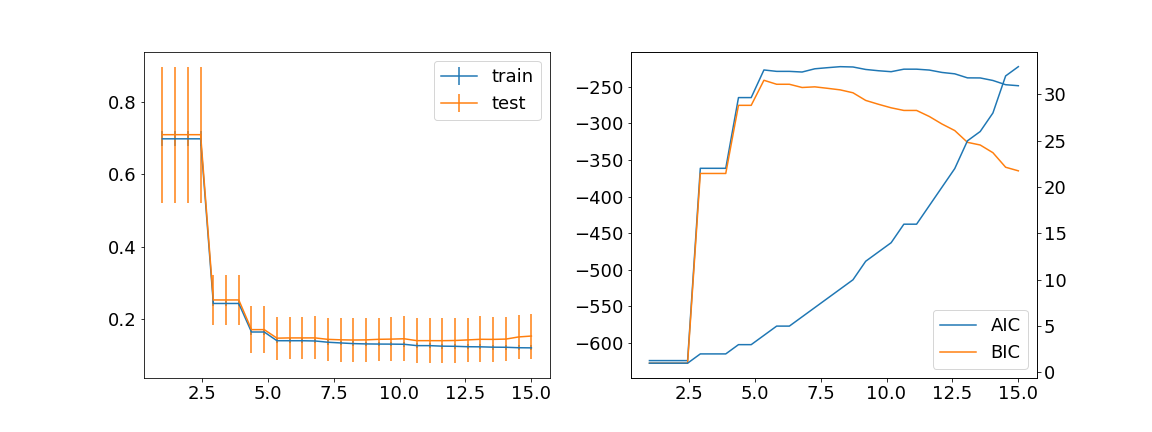
\includegraphics[width = 0.8\textwidth]{figures/cutoff_scan.png}
    \caption{Caption}
    \label{fig:cutoff_scan}
\end{figure}


Next we are performing feature selection and in figure \ref{fig:Lasso_scan} the CV-score together with the BIC and AIC, when we used LASSO, are presented as a function of the hyper parameter $\beta$. We now observe as before that there is a maximum for the BIC, which can be used to select the best value for the hyper parameter ca ???. Also AIC seems to suggest that this value of $\beta$ leads to a good model however AIC equals this to the models with lower hyper parameters i.e models with more parameters. We can also see from the CV-score that the MSE for the testing data has a minimum at around the same value of $\beta$ as BIC had a maximum. For lower values of $\beta$ (many non-zero parameters) the testing error start to rise from the training error once again indicating over fitting. We can thus conclude that the increase in maximum likelihood that compensate for the increasing number of parameters in AIC comes from over fitting and we should choose $\beta$ such we maximizes the BIC and minimizes the testing error i.e $\beta = $???. This value for the hyper parameter also leads to $ $??? number of non-zero parameters in the model. 

In figure \ref{fig:ARDR_scan} we can see the CV-score, BIC and AIC as a function of $1/\lambda$ when ARDR was used. The result have some similaryties to the previous but also some differences. In
\begin{figure}[H]
    \centering
    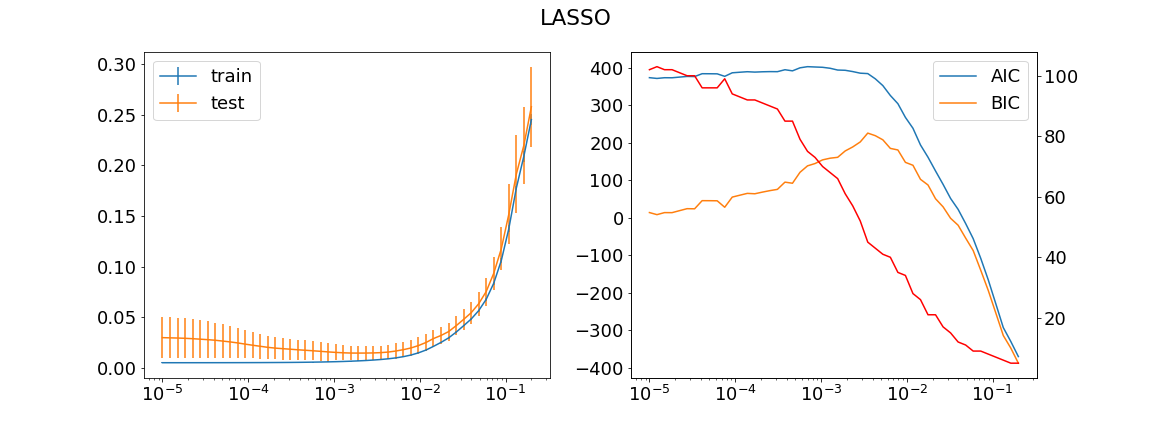
\includegraphics[width = 0.8\textwidth]{figures/LASSO_scan.png}
    \caption{Caption}
    \label{fig:Lasso_scan}
\end{figure}

\begin{figure}[H]
    \centering
    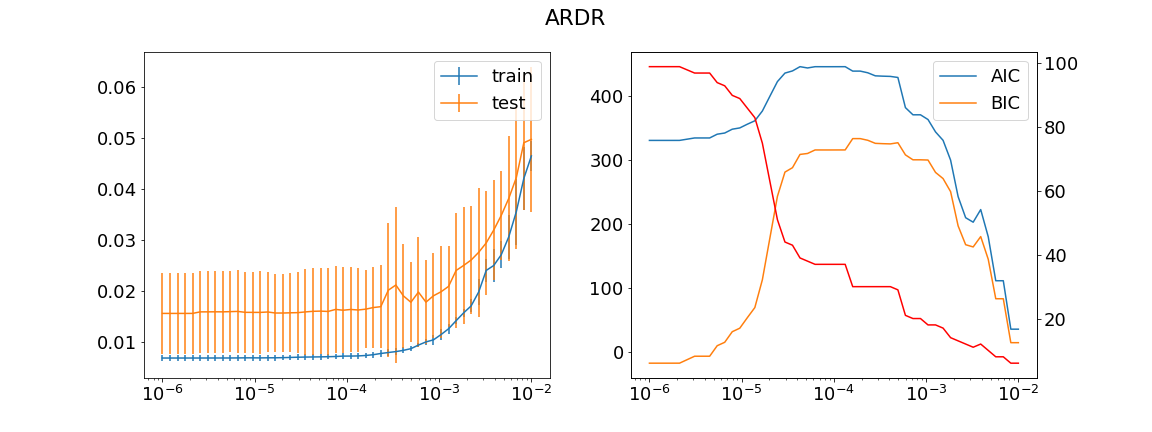
\includegraphics[width = 0.8\textwidth]{figures/ARDR_scan.png}
    \caption{Caption}
    \label{fig:ARDR_scan}
\end{figure}

\begin{figure}[H]
    \centering
    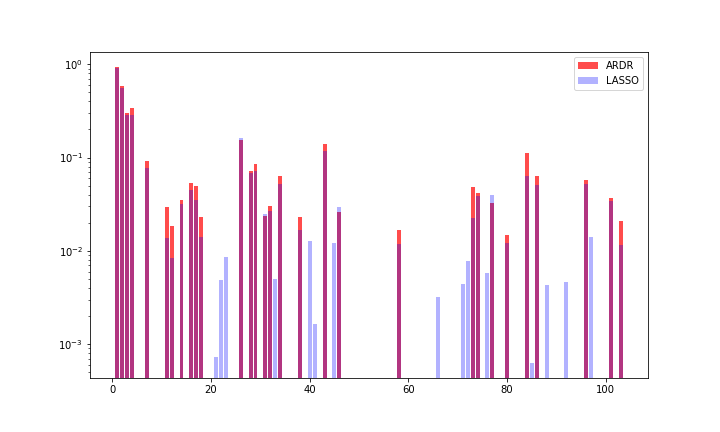
\includegraphics[width = 0.8\textwidth]{figures/lasso_ardr_weights_overlap.png}
    \caption{Caption}
    \label{fig:weights_overlap}
\end{figure}

\subsection[Task 2]{Task 4: Bayesian Cluster expansion}

The MCMC sampling was found to converge well with the settings described above, yielding an acceptance ratio of $\sim 0.2$ for all walkers, and resulted in the posterior distributions for the ECIs $\mathbf{J}$ given in figure \ref{fig:bayes_eci}.

\begin{figure}[ht]
    \centering
    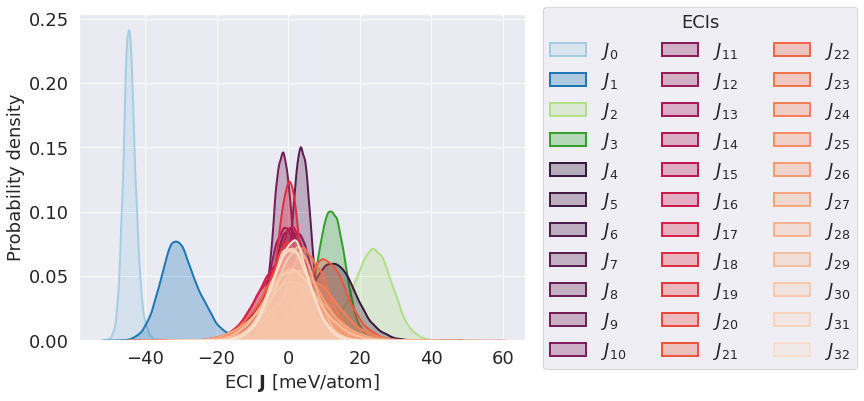
\includegraphics[width=0.7\textwidth]{figures/task4_ecis.png}
    \caption{Sampled posterior distributions for the ECIs $\mathbf{J}$ for the given cutoff values. Note that most ECIs are centered around zero, with only the first few (mainly $J_1--J_4$) being centered around non-zero values. This could imply that mainly a few cluster types contribute to the mixing energy, with most of the available cluster types for these cutoff values contributing very little.}
    \label{fig:bayes_eci}
\end{figure}
Note that the distributions are given a different hue depending on which $J_\alpha$ they correspond to; larger $\alpha$ corresponds to a darker hue. We observe that all ECIs $J_\alpha$ are somewhat Gaussian in shape, and that almost all are centered around zero. Hence, one cannot draw a clear conclusion on the magnitude of these ECIs; a mean \textit{a posteriori} estimate would set them to zero. However, there are some ECIs which are centered with a mean other than zero. These ECIs correspond mostly to clusters with low $\alpha$, with the most prominent being $J_1$, $J_2$, $J_3$ and $J_4$. Thus one could draw the conclusion that the primary contributions to the mixing energy for these cutoff values comes from only a few cluster types, with most most of the allowed clusters types contributing very little. 

\begin{figure}[ht]
    \centering
    \begin{subfigure}{.5\textwidth}
          \centering
          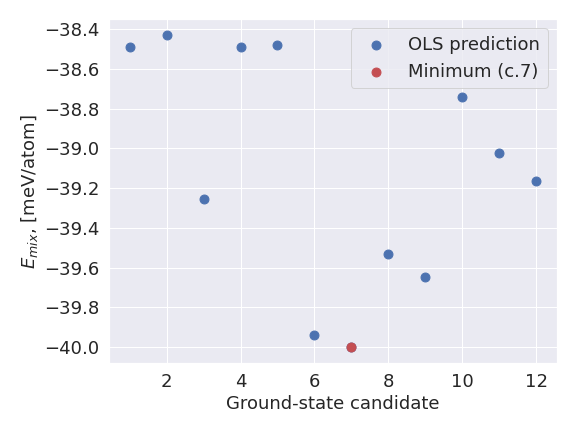
\includegraphics[width=0.9\linewidth]{figures/OLS_prediction.png}
          \caption{OLS ground state predictions.}
          \label{fig:ols_ground}
    \end{subfigure}%
    \begin{subfigure}{.5\textwidth}
          \centering
          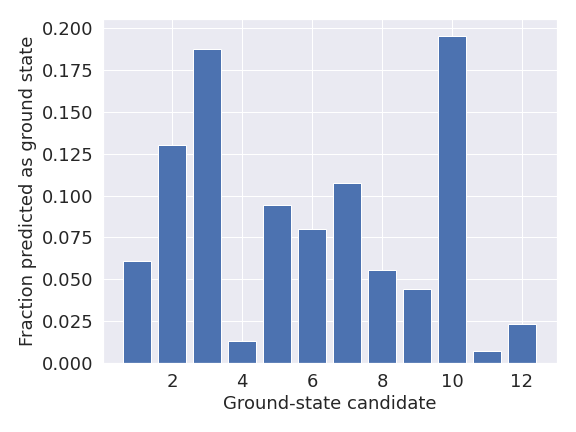
\includegraphics[width=0.9\linewidth]{figures/task4_bayes_hist.png}
          \caption{Bayesian ground state predictions.}
          \label{fig:bayes_ground}
    \end{subfigure}
    \caption{Ground state predictions for OLS and the Bayesian cluster expansion. Note the small scale on the y-axis in figure \ref{fig:ols_ground}, which implies that all the cluster candidates are fairly similar.}
    \label{fig:ground_predict}
\end{figure}

Moving on to the predictions for which cluster among the candidates corresponds to the ground state. The predictions made by OLS and Bayesian cluster expansion are given in figures \ref{fig:ols_ground} and \ref{fig:bayes_ground} respectively. OLS predicts cluster candidate 7 to be the ground state, closely followed by cluster candidate 6. Note however the small differences in predicted cluster energy for all 12 candidates, which indicates that the clusters are fairly similar. This is further indicated by the Bayesian cluster predictions, in which multiple different candidates are predicted to be the ground state with fairly high frequency. The four most often predicted candidates are in descending order clusters 10, 3, 2 and 7. We also note that the posterior predictive distributions of the mixing energies for the various cluster candidates, given in figure \ref{fig:bayes_dist}, overlap with almost no discernible difference. The conclusion from the Bayesian analysis of which candidate corresponds to the ground state is thus much more inconclusive than in the case of OLS; we advocate that no conclusion can be drawn from the data. This difference between OLS and a Bayesian analysis exemplifies the exemplifies the importance of using methods that estimate the uncertainty in the prediction, and not simply makes a ``certain'' prediction. With this being said, it is not always necessary to do a full Bayesian analysis. For instance, one could instead splitn the available data $\mathcal{D}$ into $k$ parts and trained $k$ different OLS models, and model averaging the predictions for the ground state candidates to obtain a mean prediction and a variance in that prediction. 

\begin{figure}[ht]
    \centering
    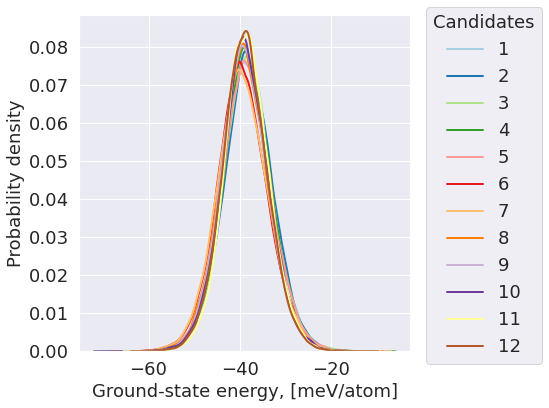
\includegraphics[width=0.7\textwidth]{figures/task4_bayes_ground.png}
    \caption{Posterior predictive distribution of the mixing energy for ground state candidates. Note that the distributions overlap to a high degree, with almost no discernible difference between the candidates. }
    \label{fig:bayes_dist}
\end{figure}

There are a few possible improvements one could make in order to improve the Bayesian analysis. First, one could add more data (perhaps from other sources), which we would expect to decrease the \textit{a posteriori} variance, which in turn could help separate the posterior predictive distributions (PPDs) for the various cluster candidates. However, since the means of the PPDs for our current amount of data in figure \ref{fig:bayes_dist} are very similar, and if we assume that our current amount of data leads to posteriors which represent the ``true'' mixing energy distributions for the candidates well, it is not certain that just adding more data would lead to a more conclusive answer. Secondly, one could improve the Bayesian model by adding a Gaussian noise with variance $\alpha^2$ to the posterior predictions, which would correspond to modelling the model uncertainty. Going down this road would probably lead to a larger variance in the PPDs, which in turn would make the results even less conclusive. Note that this would be a good thing, since the model would be more representative of the uncertainty in the actual data. 



% OLS leads to overconfident conclusion - Bayesian approach yields a much less "cleer cut" conclusion. All distributions overlap.
% How could one improve the Bayesian approach? One way could be through more data; by adding more data the predictions would be made much more narrow. => Good or bad, depending on the quality of the data. 

\printbibliography

\end{document}
